\chapter{THIẾT KẾ HỆ THỐNG}
\section{Lựa chọn công cụ}

\paragraph{}
Rust là ngôn ngữ lập trình hệ thống mới nổi với nhiều ưu thế đảm bảo an toàn bộ nhớ, an toàn về luồng kèm theo các công cụ hỗ trợ mạnh mẽ, vì vậy nhóm sử dụng Rust làm ngôn ngữ lập trình chính.

\paragraph{}
Do lập trình giao diện trên Rust còn khó khăn, nhóm thực hiện phần mềm trên môi trường web tĩnh, các trang html được viết dưới dạng khung mẫu hỗ trợ bởi thư viện Tera.

\paragraph{}
Giao tiếp giữa cơ sở dữ liệu SQLite với chương trình được thực hiện qua thư viện sqlx. Sqlx là một thư viện hỗ trợ kết nối tới nhiều cơ sở dữ liệu khác nhau hỗ trợ cú pháp được phân tích ngay trong thời điểm biên dịch chương trình, giúp giảm thiếu lỗi khi lập trình.

\paragraph{}
Thuật toán X25519 được sử dụng cho trao đổi khóa \gls{ecdh} do nó được coi là an toàn. Mã hóa đối xứng sử dụng thuật hệ mã ChaCha20Poly1305. Hàm băm BLAKE2s được sử dụng cho việc sinh khóa.

\section{Thiết kế phần mềm}

\subsection{Thiết kế tổng thể}

\paragraph{}
Các thành phần của phần mềm bao gồm:
\begin{enumerate}
	\item Thành phần quản lý: nơi lưu trữ dữ liệu phân quyền, dữ liệu, điều khiển chương trình, thực hiện các thao tác mã hóa, sinh khóa gọi chung là phần mềm.
	\item Thành phần mã hóa, giải mã: thực hiện \gls{encrypt} dữ liệu trên các ô khi lưu trữ và giải mã khi có yêu cầu từ người dùng hợp lệ. Dữ liệu được \gls{encrypt} sử dụng hệ thống mã hóa công khai, cho phép nhiều người dùng có thể đọc dữ liệu với khóa riêng và cho các người dùng khác có thể đọc được dữ liệu sau khi cập nhật mới.
	\item Thành phần sinh khóa: thực hiện tạo \gls{key} \gls{encrypt} cho người dùng. Mỗi người dùng có một cặp \gls{key} công khai-bí mật, cặp khóa này được sinh bởi tên và mật khẩu nhập bởi người dùng và người dùng chịu trách nhiệm quản lý mật khẩu này.
\end{enumerate}
\begin{figure}[H]
	\centering
	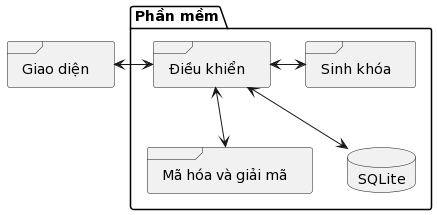
\includegraphics{images/component-diagram.png}
	\caption{Các thành phần của phần mềm}
\end{figure}

\subsection{Thành phần sinh khóa}

\paragraph{}
Tên và mật khẩu được gắn liền với mỗi người dùng và khóa giải mã, mã hóa được tạo ra từ 2 tham số này. Khóa bí mật $s$ tính theo công thức $s=h(n+p)$ trong đó $h$ là hàm băm BLAKE2s, $n$ là tên người dùng, $p$ là mật khẩu, + là phép nối chuỗi.

\paragraph{}
Khóa công khai $k$ được tính theo thuật toán \gls{ecdh}: $k=sG$.

\subsection{Thành phần mã hóa - giải mã}

\paragraph{}
Với mỗi đoạn dữ liệu cần mã hóa, kỹ thuật \gls{asymmetric cipher} được sử dụng dựa trên thuật toán X25519. Khi cần cập nhật dữ liệu, khóa bí mật tạm thời $s_e$ được tạo ngẫu nhiên, đối với mỗi người dùng với khóa công khai $k_x$, bí mật chung $Sh_x$ được tính bằng $Sh_x=s_ek_x$. Bí mật chung $Sh_x$ sử dụng để tính khóa mã hóa $Kc_x$ bằng cách đưa vào hàm băm $h$: $Kc_x=h(Sh_x)=h(s_ek_x)$. Khóa công khai tạm thời $k_e$ được lưu cùng với dữ liệu mã hóa. Dữ liệu $m$ cho từng người dùng $x$ được mã hóa bởi khóa $Kc_x$ qua hàm mã hóa $C$: $t_x = E(Kc_x, m)$. Các cặp khóa công khai, và dữ liệu mã hóa $(k_x, t_x)$ được lưu kèm cùng với khóa công khai tạm thời $k_e$ tạo thành bộ dữ liệu mã hóa:
$T = (k_e, ((k_1, t_1), ..., (k_n, t_n)))$ với $t_x=E(h(s_ek_x), m) = E(h(s_xk_e), m)$

\paragraph{}
Quá trình giải mã được thực hiện bởi người dùng $x$ có khóa bí mật $s_x$. Từ tập $T$, người dùng $x$ lấy khóa công khai tạm thời $k_e$, và tìm thông điệp $t_x$ thông qua khóa $k_x$ của họ. Khóa giải mã $Kc_x$ được tính $Kc_x = h(s_xke)$ và được sử dụng để giải mã thông điệp $m$ từ bản mã $t_x$: $m=D(h(s_ek_x), t_x$.

\subsection{Thành phần quản lý}

\paragraph{}
Thông tin tên và khóa công khai của người dùng được phần mềm lưu trữ trong bản smask\_role:
\begin{table}[H]
	\centering
	\caption{Bảng người dùng smask\_role}
	\begin{tabular}{|c|c|c|}
		\hline
		\textbf{Tên cột} & \textbf{Kiểu dữ liệu} & \textbf{Chú thích} \\
		\hline
		\textbf{smask\_role} & text & Tên người dùng\\
		\hline
		\textbf{smask\_key} & blob & Khóa công khai \\
		\hline
	\end{tabular}
\end{table}

\paragraph{}
Các cột và bảng được có quyền truy cập bởi người dùng được lưu trong bảng smask\_role\_table và smask\_role\_column với smask\_key là khóa công khai của người dùng có quyền hạn:
|
\begin{table}[h]
	\centering
	\caption{Bảng thông tin phân quyền cho bảng}
	\begin{tabular}{|c|c|c|}
		\hline
		\textbf{Tên cột} & \textbf{Kiểu dữ liệu} & \textbf{Chú thích} \\
		\hline
		\textbf{smask\_table} & text & Tên bảng\\
		\hline
		\textbf{smask\_key} & blob & Khóa công khai \\
		\hline
	\end{tabular}
\end{table}

\begin{table}[h]
	\centering
	\caption{Bảng thông tin phân quyền cho cột}
	\begin{tabular}{|c|c|c|}
		\hline
		\textbf{Tên cột} & \textbf{Kiểu dữ liệu} & \textbf{Chú thích} \\
		\hline
		\textbf{smask\_column} & text & Tên cột\\
		\hline
		\textbf{smask\_table} & text & Tên bảng\\
		\hline
		\textbf{smask\_key} & blob & Khóa công khai \\
		\hline
	\end{tabular}
\end{table}

\paragraph{}
Dữ liệu được lưu trong các cột có cấu trúc: 

\begin{verbatim}
	struct Cell (ephemeral_pubkey, Map<user_pubkey, cipher_text>)
\end{verbatim}
Trong đó: ephemeral\_pubkey là \gls{key} công khai tạm thời, user\_pubkey là \gls{key} công khai của người dùng và cipher\_text là dữ liệu $m$ được \gls{encrypt} của ô đối với người dùng được chọn. 